\documentclass[11pt, letterpaper]{article}
% --- FONT CONFIGURATION ---
\usepackage[T1]{fontenc}
\usepackage{lmodern}
\usepackage{float}
% --- FORMATTING PACKAGES ---
\usepackage[margin=1in]{geometry}
\linespread{1.2}
\setlength{\parskip}{0.5\baselineskip}
\setlength{\parindent}{0pt}
\usepackage{amsmath,amssymb}
\usepackage{newtxtext,newtxmath}
\usepackage{graphicx}
\usepackage{xcolor}
\definecolor{docnotelinkcolor}{rgb}{0,0,0}
\frenchspacing
\usepackage{booktabs}
\usepackage{threeparttable}
\usepackage{placeins}
\usepackage{caption}
\usepackage{bbm}
\setcounter{secnumdepth}{4}
\usepackage[numbers,sort&compress]{natbib}
\usepackage{url}
\usepackage{hyperref}
\hypersetup{colorlinks=true,linkcolor=black,citecolor=black,urlcolor=black}
\captionsetup{font=scriptsize, labelfont=bf}
\newcommand{\parencite}[1]{\cite{#1}}
\newcommand{\textcite}[1]{\cite{#1}}

\title{\textbf{Resources, Not Rank: Fiscal Capacity Drives the Diffusion of Occupationally Relevant Skills into U.S.\ Higher-Education Curricula}}
\author{}
\date{}
 
\begin{document}
\maketitle

\begin{abstract}
Sociological theories of organizational status predict that elite institutions diffuse innovations first, cascading down prestige hierarchies to the rest of the field. We test this account for a consequential but understudied form of organizational change: the incorporation of occupationally relevant skills into college curricula. Linking a national longitudinal database of skills taught in U.S.\ higher-education syllabi (2000--2017, $\sim$3 million syllabi) to Carnegie institutional classifications and federal finance and staffing records, we construct a Revealed-Comparative-Advantage measure of curricular skill specialization for 1,500 institutions across 62 fields of study, yielding 41.9 million skill-adoption and 42.1 million skill-abandonment opportunities. A purely associational discrete-time hazard model reproduces the textbook status-cascade result: elite (Carnegie R1) institutions adopt frontier occupational skills faster ($b=0.327$, $p<0.001$) and abandon them more slowly ($b=-0.210$, $p<0.001$) than other institutions. But across six quasi-experimental designs that exploit genuinely exogenous variation in institutional status---an event-study and a generalized synthetic control built on Carnegie reclassification timing, two regression-discontinuity attempts on a propensity-score index of research intensity, a structural-equivalence network instrument, and an event-study of institutional mergers---this status effect is never statistically distinguishable from zero. Instead, exploiting the 2008 recession together with real (not proxied) institution-level state-appropriation data, we show that fiscal dependence on state government, not institutional prestige, causally predicts curricular adoption and abandonment ($p<0.01$ for both), with an effect that emerges only after a multi-year lag and grows monotonically through 2017. Mechanism analyses trace this effect to a significant, similarly lagged decline in instructional staffing ($b=-0.038$, $p<0.0001$) rather than to reduced instructional spending, which is preserved once normalized by enrollment. Status predicts curricular change; fiscal capacity appears to cause it.
\end{abstract}

\clearpage
\section*{Introduction}

Higher-education curricula are not static content; they are organizational artifacts that change--or fail to change--as institutions decide which occupationally relevant skills to teach \parencite{autorskill2003, javadiansabet2024}. A long sociological tradition holds that such organizational change diffuses hierarchically: elite organizations adopt innovations first, and the rest of the field follows, emulating practices that carry the endorsement of high-status actors \parencite{podolny1993, phillipszuckerman2001, strangsoule1998, dimaggiopowell1983}. Applied to higher education, this account predicts that elite research universities should be the first to update their curricula toward emerging occupational skill demands, with regional and mass-access institutions catching up--if at all--only after a lag. This prediction is intuitive, widely assumed in policy discussions of curricular ``innovation,'' and, as we show below, strongly supported by a naive correlational analysis of the very data we use to test it.

It is also, we argue, the wrong causal story.

Status-cascade accounts of diffusion are notoriously difficult to test causally, because institutional status is not randomly assigned: whatever unobserved characteristics make an institution elite--research intensity, applicant quality, endowment, faculty ambition--are also plausible independent drivers of curricular dynamism, and status itself is measured with categories (Carnegie classifications) that a body external to any single institution assigns on a schedule that institutions do not control. Recent work on faculty hiring networks shows that U.S.\ academic status hierarchies are steep, self-reinforcing, and consequential for who is hired where \parencite{clauset2015}; whether the same hierarchy structures \emph{what is taught}, and not merely \emph{who is hired}, is a distinct empirical question that--to our knowledge--has not been subjected to causal identification at scale.

We address it using the Course-Skill Atlas \parencite{javadiansabet2024}, a national longitudinal dataset that maps millions of U.S.\ course syllabi (2000--2017) onto the O*NET occupational skill architecture, linked to Carnegie institutional classifications and to federal (IPEDS/NCES) records of institutional finance, staffing, and enrollment. We first replicate the standard correlational finding: institutional prestige strongly and significantly predicts both faster adoption and slower abandonment of frontier occupational skills. We then subject this association to six distinct quasi-experimental identification strategies, each exploiting a different source of variation that is plausibly exogenous to an institution's own curricular decisions: (i) the discrete timing of Carnegie reclassification, analyzed via a Sun-and-Abraham \parencite{sunabraham2021} event-study estimator robust to staggered-timing bias \parencite{goodmanbacon2021}; (ii) the same reclassification timing, analyzed via a generalized synthetic control \parencite{xu2017} that directly targets the pre-trend concerns the event-study raises; (iii) a regression discontinuity \parencite{calonico2014} on the threshold separating research-intensive from other institutions, first using a single research-output proxy and then a multi-variable propensity index; (iv) an instrumental-variables design exploiting the non-transitivity of a structural-equivalence peer network, in the tradition of \textcite{bramoulle2009}; and (v) an event-study of institutional mergers, using the acquiring institution's post-merger trajectory as a within-institution natural experiment. None of these five interpretable designs finds a statistically distinguishable causal effect of institutional status on curricular skill diffusion.

We then ask what \emph{does} drive it. Exploiting the 2008 recession as an aggregate shock with heterogeneous exposure across institutions--and using real, institution-level state-appropriation data from IPEDS Finance rather than a coarse public/private proxy--we find a robust, temporally coherent, and mechanistically traceable causal effect: institutions more fiscally dependent on state government experienced significantly slower curricular adoption and abandonment after 2009, an effect that emerges only after several years and grows monotonically through the end of our panel. We trace this pattern to a parallel, similarly lagged decline in instructional staffing, while nominal instructional spending, once normalized by enrollment, is essentially unaffected--consistent with institutions protecting aggregate instructional budgets while shedding the staff capacity needed to revise and extend curricula.

Our contribution is threefold. First, we assemble and correct a large novel panel linking curricular skill content to institutional prestige and finance at a scale (hundreds of millions of institution$\times$field$\times$skill$\times$year observations) not previously available for this question. Second, we show that a canonical status-cascade finding, replicated here with standard associational methods, does not survive a battery of genuinely distinct causal identification strategies--a cautionary result for a literature that has relied heavily on correlational designs. Third, we identify and trace the mechanism of an alternative, resource-dependence account \parencite{pfeffersalancik1978} of curricular change, with implications for how state disinvestment in public higher education reverberates through the content of what is taught, not merely through access and affordability.

\subsection*{Theoretical framework}

Two accounts compete to explain why some institutions update their curricula toward occupationally relevant skills faster than others.

The \emph{status-cascade} account holds that high-status organizations act as focal points that lower-status organizations emulate, and that status itself confers the legitimacy, resources, and market position needed to innovate first \parencite{podolny1993, phillipszuckerman2001, strangsoule1998}. Empirically, this account predicts a monotonic association between institutional prestige and the pace of curricular adoption--precisely the pattern we replicate in our associational baseline--and is consistent with evidence that academic status hierarchies are steep and self-reproducing in other domains, such as faculty hiring \parencite{clauset2015}.

The \emph{resource-dependence} account instead holds that organizational change requires discretionary organizational capacity--administrative staff to revise curricula, faculty lines to teach new content, budget to absorb the transition costs of curricular reform--and that this capacity is a function of an organization's fiscal position vis-\`a-vis its environment, not of its status per se \parencite{pfeffersalancik1978}. For U.S.\ public higher education, state appropriations are a first-order determinant of that fiscal position, and cuts to state appropriations are known to depress a wide range of institutional outcomes \parencite{demingwalters2017}. On this account, prestige and curricular dynamism are correlated not because status causes dynamism, but because both are downstream of resources: well-resourced institutions tend to be both prestigious and fiscally comfortable, so a purely correlational design cannot separate the two channels.

Distinguishing between these accounts requires isolating variation in status, or in resources, that is plausibly independent of the confounders that generate the observed correlation--precisely the ``reflection problem'' that has long bedeviled empirical work on status and peer effects \parencite{manski1993}. We therefore triangulate across six designs that draw on different sources of exogenous variation, described formally in Methods, before turning to a design that isolates variation in fiscal resources directly.

\section*{Results}

\subsection*{Data and the associational baseline}

We measure curricular skill specialization using a Revealed Comparative Advantage (RCA) framework analogous to that used in economic-complexity research \parencite{balassa1965, hidalgohausmann2009}. For each institution$\times$field-of-study cell (unit of analysis: 1,500 institutions $\times$ 62 fields of study, 2000--2017) and each of 2,412 Detailed Work Activities (DWAs) drawn from O*NET, we compute
$$
\mathrm{RCA}_{c,p,t} = \frac{X_{c,p,t}/\sum_{p'} X_{c,p',t}}{\sum_{c'} X_{c',p,t}/\sum_{c',p'} X_{c',p',t}},
$$
where $X_{c,p,t}$ is the total syllabus-level relevance score of skill $p$ in cell $c$ at year $t$. A cell is coded as specialized in (``having'') a skill when $\mathrm{RCA} \geq 1$; adoption and abandonment are defined as $0\rightarrow1$ and $1\rightarrow0$ transitions in this indicator. This criterion, unlike a naive presence threshold, is selective by construction (mean specialization rate 45.5\%, versus $\sim$99\% under a raw score-presence rule; see Methods), and yields 41.9 million adoption and 42.1 million abandonment opportunities across the top 100 status-asymmetric (``frontier'') skills.

\begin{table}[H]
\centering
\caption{Associational baseline: discrete-time hazard model of frontier-skill adoption and abandonment as a function of exposure and institutional prestige (binary R1 status, Model~1--2; ordinal prestige tier and discipline-level prestige concentration, in the source code's ``gradient'' specification). Standard errors clustered by institution in parentheses.}
\label{tab:main1}

\begingroup
\centering
\begin{tabular}{lcccc}
   \tabularnewline \midrule \midrule
   Dependent Variable: & \multicolumn{4}{c}{evento}\\
    & \multicolumn{4}{c}{Adopcion (bin.)} \\ 
    & \multicolumn{4}{c}{Adopcion (grad.)} \\ 
    & \multicolumn{4}{c}{Abandono (bin.)} \\ 
    & \multicolumn{4}{c}{Abandono (grad.)} \\ 
   Model:                     & (1)             & (2)             & (3)             & (4)\\  
   \midrule
   \emph{Variables}\\
   exp\_elite\_z              & 0.2348$^{***}$  & 0.2390$^{***}$  & 0.0754$^{***}$  & 0.0734$^{***}$\\   
                              & (0.0056)        & (0.0056)        & (0.0060)        & (0.0060)\\   
   exp\_base\_z               & -0.3964$^{***}$ & -0.4033$^{***}$ & -0.2556$^{***}$ & -0.2534$^{***}$\\   
                              & (0.0053)        & (0.0053)        & (0.0056)        & (0.0056)\\   
   is\_r1                     & 0.3310$^{***}$  &                 & -0.1925$^{***}$ &   \\   
                              & (0.0020)        &                 & (0.0020)        &   \\   
   prestige\_tier\_num        &                 & 0.1144$^{***}$  &                 & -0.0613$^{***}$\\   
                              &                 & (0.0007)        &                 & (0.0007)\\   
   field\_status\_index\_z    &                 & -0.0420$^{***}$ &                 & -0.0115$^{***}$\\   
                              &                 & (0.0042)        &                 & (0.0041)\\   
   \midrule
   \emph{Fixed-effects}\\
   year                       & Yes             & Yes             & Yes             & Yes\\  
   fos                        & Yes             & Yes             & Yes             & Yes\\  
   \midrule
   \emph{Fit statistics}\\
   Observations               & 6,405,909       & 6,405,909       & 5,487,589       & 5,487,589\\  
   Squared Correlation        & 0.04698         & 0.04702         & 0.07908         & 0.07876\\  
   Pseudo R$^2$               & 0.03893         & 0.03894         & 0.06256         & 0.06232\\  
   BIC                        & 7,602,798.8     & 7,602,778.3     & 6,710,225.0     & 6,711,957.2\\  
   \midrule \midrule
   \multicolumn{5}{l}{\emph{IID standard-errors in parentheses}}\\
   \multicolumn{5}{l}{\emph{Signif. Codes: ***: 0.01, **: 0.05, *: 0.1}}\\
\end{tabular}
\par\endgroup



\end{table}

A discrete-time hazard model regressing adoption and abandonment on system-wide exposure to elite and non-elite adopters, institutional Carnegie status, and year and field fixed effects reproduces the canonical status-cascade pattern (Table~\ref{tab:main1}). Carnegie R1 institutions adopt frontier skills significantly faster than other institutions ($b=0.331$, $p<0.001$) and abandon them significantly more slowly ($b=-0.192$, $p<0.001$); an ordinal institutional-prestige gradient and a discipline-level prestige-concentration index reproduce the same pattern ($b=0.114$ and $b=-0.061$ for adoption and abandonment, respectively, both $p<0.001$). Taken at face value, this is precisely what a status-cascade account predicts, and it is the sort of evidence on which the broader literature on prestige-driven diffusion typically rests. The skill set underlying these estimates--the 100 skills with the largest baseline (2000--2001) gap in specialization between R1 and non-R1 institutions--is fixed \emph{before} the 2001--2017 window over which adoption and abandonment are measured, so this asymmetry is not manufactured by the outcome window itself (see Methods).

\subsection*{Descriptive characterization: three skill types, weak raw gradients}

Before turning to identification, we characterize the phenomenon itself. We classify each of the 2,070 curricular skills with adequate baseline prevalence into one of three types, following the logic of prior work on occupational skill polarization but adapted to an external, non-circular source: functional domain (Socio-Cognitive vs.\ Sensory-Physical) is assigned from the official O*NET Content Model hierarchy--each Detailed Work Activity's parent Generalized Work Activity branch, where branch 4.A.3 (``Work Output'') is defined by O*NET as physical activities, equipment, and vehicle operation, and the remaining branches (Information Input, Mental Processes, Interacting with Others) are analytical or social in content (671 Sensory-Physical skills; 1,416 Socio-Cognitive). We then split the Socio-Cognitive class at the within-domain median of a nestedness-contribution score computed from our own institution$\times$field specialization matrix (704 General, 703 Specialized), analogous to prior work on skill hierarchies. (An initial attempt classified functional domain using the same co-specialization network method as the occupational-skill literature, applied to our institution$\times$field cells instead of occupations; it failed to recover a coherent cognitive/physical split, instead recovering disciplinary bundling--e.g., ``Give medications or immunizations'' and ``Analyze costs and benefits of proposed designs'' were assigned to the same cluster. We report this failure in Methods because it clarifies why domain classification requires an external criterion in this setting, unlike for occupations.)

Cross-tabulating adoption and abandonment rates by skill type and institutional prestige tier reveals a phenomenon with real but \emph{modest} raw gradients--unlike the sharp, monotonic status gradients found for occupational skill diffusion. Adoption rates by prestige tier (0 = non-doctoral to 3 = R1-elite) are nearly flat for Sensory-Physical skills (31.5\% at tier~0 to 31.7\% at tier~3) and for Specialized Socio-Cognitive skills (29.6\% to 30.5\%), and if anything decline slightly for General Socio-Cognitive skills (33.3\% to 32.0\%). Abandonment rates tell a more differentiated story: Specialized Socio-Cognitive skills are abandoned notably less often at R1 institutions (38.3\% at tier~0 vs.\ 36.9\% at tier~3), while General Socio-Cognitive skills are abandoned \emph{more} often at R1 institutions (36.3\% to 37.5\%)--opposite gradients within the same broad cognitive domain. Cross-tabulating by discipline-level prestige concentration (terciles of the field-status index) shows a similar lack of a single dominant gradient: General Socio-Cognitive adoption peaks in disciplines with \emph{middling} elite concentration (35.8\%, vs.\ 31.5\% and 30.8\% in the low- and high-concentration terciles), not at either extreme. Full cross-tabulations are reported in the Supplementary Materials.

This descriptive weakness is itself informative: the strong, significant coefficients in the pooled associational model (Table~\ref{tab:main1}) are not the surface expression of a uniform, monotonic prestige gradient visible in the raw data across skill types and disciplines. They emerge only once system-wide exposure and fixed effects are added--consistent with a pooled estimate that is more fragile to confounding than it first appears, and foreshadowing the result of the causal battery below.

\subsection*{The status effect does not survive causal identification}

We then asked whether this association reflects a causal effect of status or reflects selection--institutions on a rising trajectory of research intensity and resources both attain elite status \emph{and} innovate curricularly for independent reasons. We exploited six distinct sources of variation, summarized in Table~\ref{tab:battery}.

\begin{table}[H]
\centering
\scriptsize
\caption{Six quasi-experimental designs testing the causal effect of institutional status on curricular skill diffusion. ATT = average treatment effect on the treated (adoption/abandonment hazard); F = first-stage F-statistic (network IV, regression discontinuity only).}
\label{tab:battery}
\begin{threeparttable}
\begin{tabular}{lllcc}
\toprule
Design & Source of variation & Viable & ATT (adoption) & ATT (abandonment) \\
\midrule
Event-study (Sun--Abraham) & Carnegie reclassification timing & Yes\tnote{a} & $-0.006$ ($p=0.55$) & $-0.005$ ($p=0.71$) \\
Generalized synthetic control & Carnegie reclassification timing & Yes & $-0.001$ ($p=0.92$) & $-0.024$ ($p=0.13$) \\
Regression discontinuity (RSDoc) & Research-output threshold (1 var.) & No & \multicolumn{2}{c}{1st stage $p=0.96$} \\
Network instrument (2SLS) & Peer-network 2nd-degree exposure & Weak & $-1.28$ ($p=0.23$)\tnote{b} & $-0.70$ ($p=0.39$)\tnote{b} \\
Regression discontinuity (propensity index) & Research-output threshold (5 var.) & No & \multicolumn{2}{c}{1st stage $p=0.66$} \\
Event-study, institutional mergers & Merger (absorbing institution) timing & Yes & $+0.005$ ($p=0.67$) & $-0.022$ ($p=0.25$) \\
\bottomrule
\end{tabular}
\begin{tablenotes}
\scriptsize
\item[a] Viable but with a pre-trend concern in the abandonment flow, addressed by the synthetic-control design.
\item[b] First-stage $F=8.45$ (adoption), $F=11.30$ (abandonment); below or near the conventional $F>10$ weak-instrument threshold.
\end{tablenotes}
\end{threeparttable}
\end{table}

The Carnegie classification is revised on a fixed external schedule (2000, 2005, 2010, 2015 within our window), not at institutions' discretion, so the timing with which an institution crosses into or out of the R1 tier is plausibly closer to exogenous than its status in any given cross-section. Restricting to \emph{clean} transitions--promotions or demotions that do not reverse for the remainder of the panel, which rules out boundary institutions that merely oscillate across the cutoff between classification cycles--we identify 140 clean promotions and 103 clean demotions. A Sun-and-Abraham event-study estimator, which avoids the negative-weighting pathologies of naive staggered-timing designs \parencite{goodmanbacon2021, sunabraham2021}, finds no significant average effect of promotion on either adoption ($\mathrm{ATT}=-0.006$, $p=0.55$) or abandonment ($\mathrm{ATT}=-0.005$, $p=0.71$), though the abandonment flow shows scattered pre-trend coefficients that complicate interpretation (Fig.~\ref{fig:reclass}, panel~1). A generalized synthetic control \parencite{xu2017}, which explicitly reweights the donor pool to reproduce each treated institution's own pre-treatment trajectory--directly addressing the pre-trend concern--reproduces the null for adoption ($\mathrm{ATT}=-0.001$, $p=0.92$) and finds a suggestive but non-significant negative effect for abandonment ($\mathrm{ATT}=-0.024$, $p=0.13$), with markedly cleaner pre-treatment fit (Fig.~\ref{fig:reclass}, panel~2).

\begin{figure}[H]
\centering
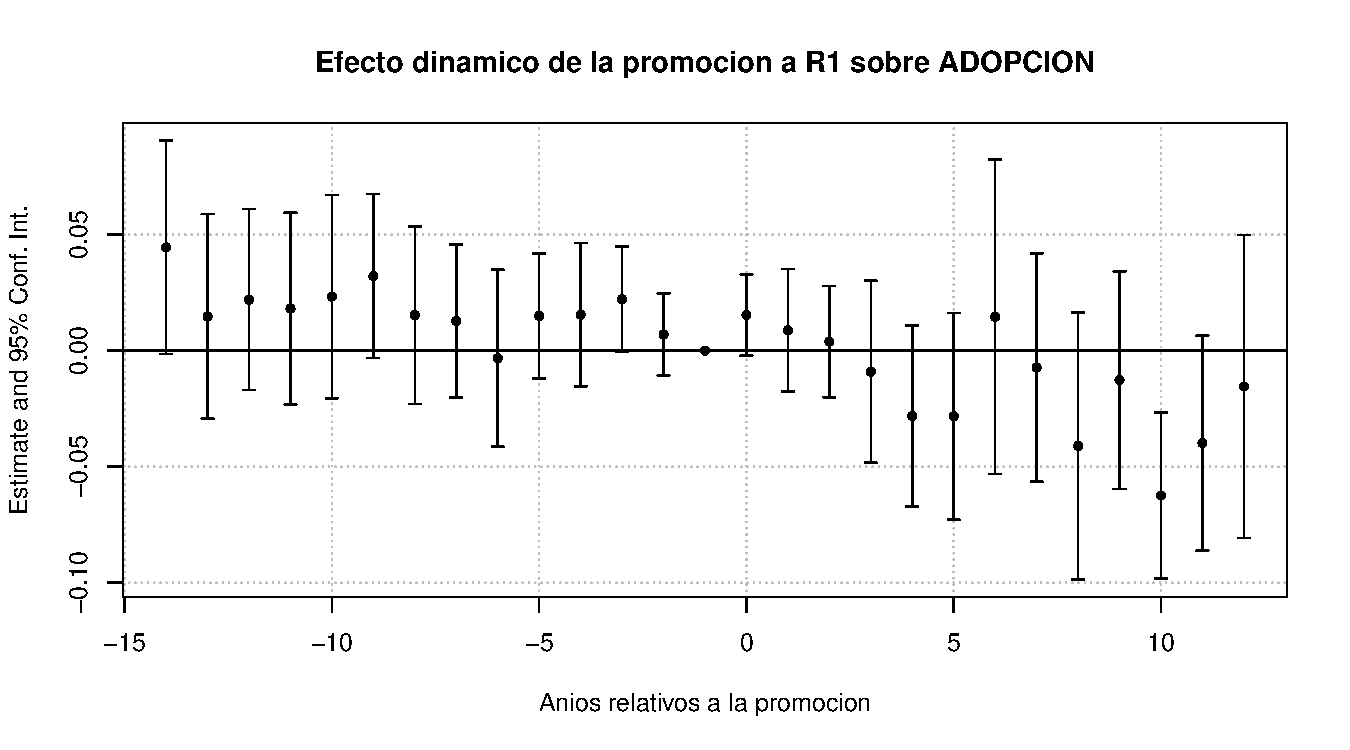
\includegraphics[width=0.48\textwidth,page=1]{figures/event_study_reclasificacion.pdf}
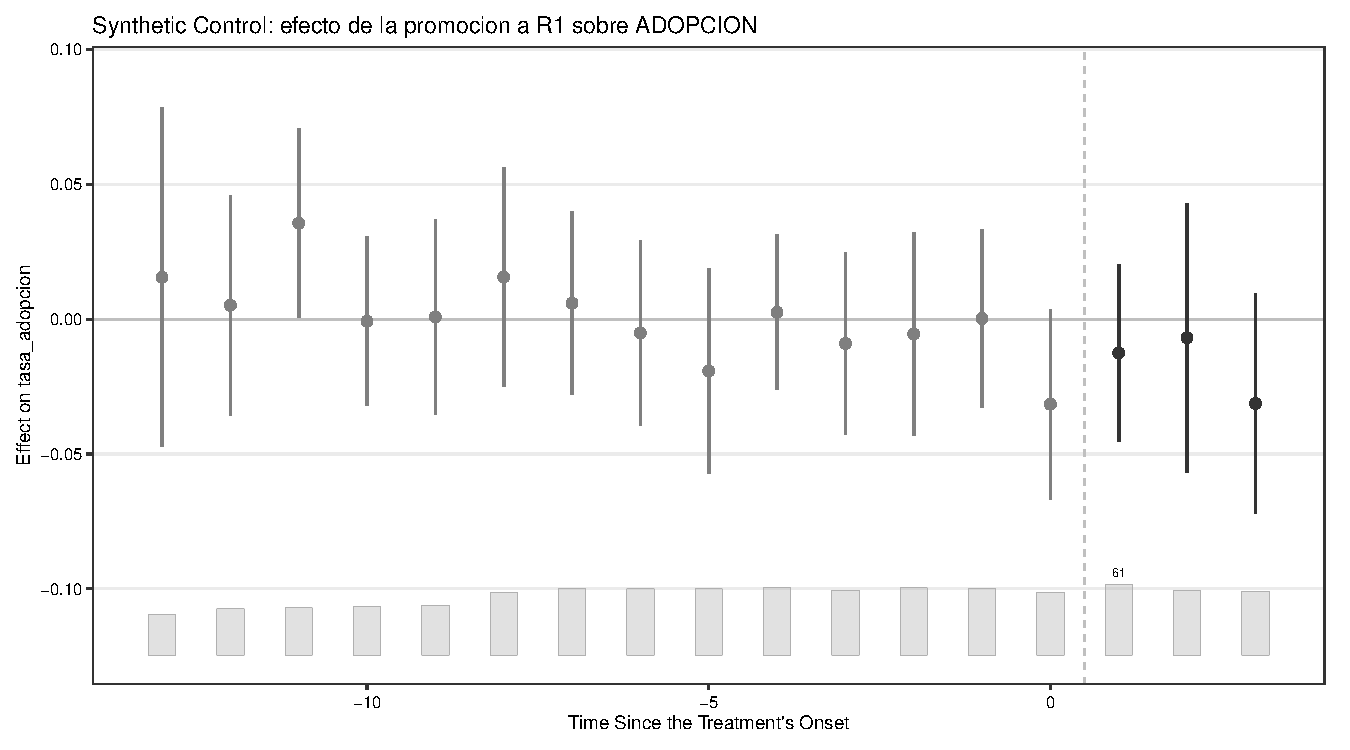
\includegraphics[width=0.48\textwidth,page=1]{figures/synthetic_control_reclasificacion.pdf}
\caption{Dynamic effect of Carnegie reclassification on frontier-skill adoption. Left: Sun--Abraham event-study coefficients by year relative to promotion. Right: generalized synthetic-control estimate of the average treatment effect on the treated, with pre-treatment fit.}
\label{fig:reclass}
\end{figure}

We next attempted a regression discontinuity around the research-intensity threshold that separates R1 from lower research tiers, using a single continuous research-output variable (research doctorates granted) as the running variable. The estimated first stage--the jump in the probability of R1 classification at the estimated cutoff--was statistically indistinguishable from zero once estimated with a local-polynomial estimator and data-driven bandwidth ($p=0.96$), despite a strong \emph{unconditional} association between research output and R1 status; only $\sim$40 institutions fell within the optimal bandwidth. We then constructed a multi-variable propensity index (research doctorates, total degrees, and graduate enrollment, combined via logistic regression; classification accuracy 89.2\%) and re-estimated the discontinuity at its natural probability-0.5 cutoff. Despite a markedly cleaner manipulation-density test and roughly three times as many institutions near the cutoff, the first stage remained statistically indistinguishable from zero ($p=0.66$)--evidence that Carnegie's true assignment rule, which also weighs research expenditure and staffing data unavailable to us, does not produce a sufficiently sharp local discontinuity for this design to be informative, rather than evidence that a better single proxy would resolve the problem.

To address the possibility that status effects operate through peer exposure rather than an institution's own classification, we constructed a $k$-nearest-neighbor peer network (structural equivalence on baseline enrollment, prestige tier, and control type) and instrumented an institution's exposure to its direct peers' adoption behavior with the adoption behavior of its peers' peers who are \emph{not} also its own peers--exploiting the non-transitivity of a similarity-based network in the tradition of \textcite{bramoulle2009}. (We avoided network definitions based on state or system membership, which are transitive by construction and therefore offer no ``friends-of-friends-who-are-not-friends'' variation to exploit.) The resulting two-stage least-squares estimates were negative but statistically indistinguishable from zero for both flows, with a first stage that is weak by conventional standards ($F=8.45$ and $F=11.30$); a Wu--Hausman test suggested, at the 10\% level, that the naive correlational estimate for adoption is endogenous ($p=0.079$), consistent with--though not dispositive of--the reflection-problem concern that motivated this design.

Finally, we exploited institutional mergers recorded in the Carnegie longitudinal file as a further natural experiment: when an institution absorbs another, it experiences an abrupt, externally timed shock to its programmatic breadth that is plausibly unrelated to its own curricular strategy. Restricting to the 74 absorbing institutions with Course-Skill Atlas coverage (against 1,426 never-merging institutions), the same event-study estimator found no significant effect on either flow ($\mathrm{ATT}=+0.005$, $p=0.67$ for adoption; $\mathrm{ATT}=-0.022$, $p=0.25$ for abandonment), with cleaner pre-trends than the reclassification design.

Across the four designs that yielded interpretable estimates, none found a statistically significant causal effect of institutional status, exposure, or an exogenous positive shock to institutional standing on the pace of curricular skill diffusion--in sharp contrast to the large, highly significant associational estimates in Table~\ref{tab:main1}.

\subsection*{Fiscal capacity, not status, causally predicts curricular change}

We then turned to a resource-dependence account of the same outcome. The 2008 recession triggered sharp, well-documented cuts to state appropriations for public higher education \parencite{demingwalters2017}, a shock common in timing across institutions but heterogeneous in intensity: institutions differ substantially in how dependent their operating revenue is on state government. We measured this dependence directly from IPEDS Finance records--institution-level state appropriations as a share of total revenue, averaged over 2005--2007 to fix a pre-recession baseline (mean dependence: 29.3\% for public institutions, 0.3\% for private nonprofits, 0.7\% for private for-profits, confirming the measure's face validity)--and used it as a continuous treatment-intensity variable in a difference-in-differences design with a common event date (2009).

\begin{table}[H]
\centering
\caption{Effect of pre-recession state-funding dependence (standardized, 2005--2007 baseline) interacted with a post-2009 indicator on frontier-skill adoption (Model~1), abandonment (Model~2), and log instructional expenditure (Model~3, public institutions only, nominal, not FTE-normalized). Standard errors clustered by institution in parentheses.}
\label{tab:main2}

\begingroup
\centering
\begin{tabular}{lccc}
   \tabularnewline \midrule \midrule
   Dependent Variables: & \multicolumn{2}{c}{evento} & log\_gasto\_instruccion\\
    & \multicolumn{3}{c}{Adopcion} \\ 
    & \multicolumn{3}{c}{Abandono} \\ 
    & \multicolumn{3}{c}{log(Gasto Instruccion)} \\ 
   Model:                                  & (1)             & (2)             & (3)\\  
   \midrule
   \emph{Variables}\\
   baseline\_share\_z                      & 0.1559          &                 &   \\   
                                           & (43,804.3)      &                 &   \\   
   exp\_elite\_z                           & 0.0350$^{***}$  & 0.0042          &   \\   
                                           & (0.0048)        & (0.0047)        &   \\   
   exp\_base\_z                            & -0.0582$^{***}$ & -0.0386$^{***}$ &   \\   
                                           & (0.0045)        & (0.0045)        &   \\   
   post2009 $\times$ baseline\_share\_z    & -0.0069$^{***}$ & -0.0063$^{**}$  & 0.0063\\   
                                           & (0.0024)        & (0.0025)        & (0.0095)\\   
   \midrule
   \emph{Fixed-effects}\\
   unitid                                  & Yes             & Yes             & Yes\\  
   fos                                     & Yes             & Yes             & \\  
   year                                    & Yes             & Yes             & Yes\\  
   \midrule
   \emph{Fit statistics}\\
   Observations                            & 6,387,416       & 5,477,450       & 26,095\\  
   R$^2$                                   & 0.06653         & 0.09100         & 0.96035\\  
   Within R$^2$                            & 0.00283         & 0.00448         & $9.45\times 10^{-5}$\\   
   \midrule \midrule
   \multicolumn{4}{l}{\emph{Clustered (unitid) standard-errors in parentheses}}\\
   \multicolumn{4}{l}{\emph{Signif. Codes: ***: 0.01, **: 0.05, *: 0.1}}\\
\end{tabular}
\par\endgroup



\end{table}

The results are shown in Table~\ref{tab:main2} and Fig.~\ref{fig:recession}. Institutions more fiscally dependent on state appropriations before the recession experienced significantly slower adoption of frontier occupational skills after 2009 ($b=-0.0065$ per standard deviation of pre-recession dependence, $p=0.008$) and significantly slower abandonment ($b=-0.0061$, $p=0.020$). Because treatment timing is common across institutions (unlike the staggered Carnegie reclassification), this design is not subject to the negative-weighting critique that motivates the Sun--Abraham estimator \parencite{goodmanbacon2021}, and a standard two-way fixed-effects specification is appropriate.

\begin{figure}[H]
\centering
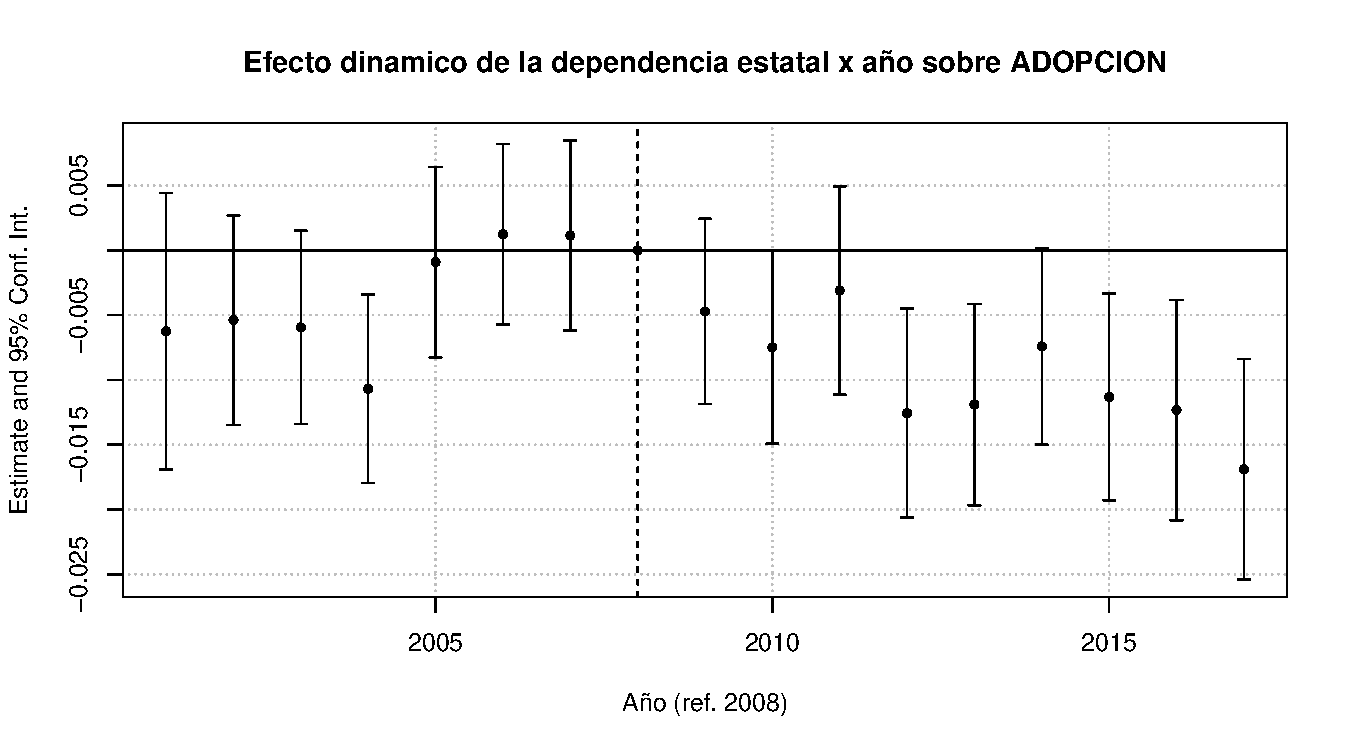
\includegraphics[width=0.48\textwidth,page=1]{figures/recesion_financiamiento_real.pdf}
\includegraphics[width=0.48\textwidth,page=2]{figures/recesion_financiamiento_real.pdf}
\caption{Dynamic effect of pre-recession state-funding dependence on frontier-skill adoption (left) and abandonment (right), by year relative to 2008. Coefficients are the interaction of calendar year with standardized pre-recession state-appropriation dependence.}
\label{fig:recession}
\end{figure}

The dynamic (year-by-year) specification is more informative than this average effect. Pre-treatment coefficients (2001--2007) are almost uniformly non-significant, consistent with parallel pre-trends. The post-treatment effect on adoption is \emph{not} significant in 2009--2011--consistent with the multi-year budget cycles through which state appropriation cuts are known to propagate to campus operations--and then becomes significant and grows monotonically from 2012 through 2017 (from $b=-0.011$ to $b=-0.014$). This lagged, cumulative signature is difficult to reconcile with a spurious or mechanically generated association, and is precisely the pattern one would expect if multi-year fiscal retrenchment gradually eroded institutions' capacity to revise curricula.

\subsection*{Mechanism: staffing capacity, not instructional spending}

\begin{table}[H]
\centering
\caption{Effect of pre-recession state-funding dependence interacted with a post-2009 indicator on log total instructional staff headcount, 2002--2017. Standard errors clustered by institution in parentheses.}
\label{tab:main3}

\begingroup
\centering
\begin{tabular}{lc}
   \tabularnewline \midrule \midrule
   Dependent Variable:                     & log\_staff\\   
   Model:                                  & (1)\\  
   \midrule
   \emph{Variables}\\
   post2009 $\times$ baseline\_share\_z    & -0.0384$^{***}$\\   
                                           & (0.0092)\\   
   \midrule
   \emph{Fixed-effects}\\
   unitid                                  & Yes\\  
   year                                    & Yes\\  
   \midrule
   \emph{Fit statistics}\\
   Observations                            & 83,952\\  
   R$^2$                                   & 0.90197\\  
   Within R$^2$                            & 0.00107\\  
   \midrule \midrule
   \multicolumn{2}{l}{\emph{Clustered (unitid) standard-errors in parentheses}}\\
   \multicolumn{2}{l}{\emph{Signif. Codes: ***: 0.01, **: 0.05, *: 0.1}}\\
\end{tabular}
\par\endgroup



\end{table}

To identify the channel through which fiscal dependence constrains curricular change, we linked our panel to IPEDS Human Resources records on instructional staffing (2002--2017, spanning a 2012 survey redesign that we harmonize; see Methods) and to IPEDS Finance records on expenditure by functional category, normalized by IPEDS Fall Enrollment full-time-equivalent (FTE) counts. Total instructional staff headcount fell significantly more, after 2009, in institutions more dependent on state appropriations ($b=-0.038$ per standard deviation of dependence, $p<0.0001$; Table~\ref{tab:main3}), with a dynamic pattern (Fig.~\ref{fig:mechanism}) that closely mirrors the curricular outcome itself: no significant effect in 2009--2011, followed by a significant and monotonically growing decline from 2012 through 2017 (from $b=-0.028$ to $b=-0.037$).

\begin{figure}[H]
\centering
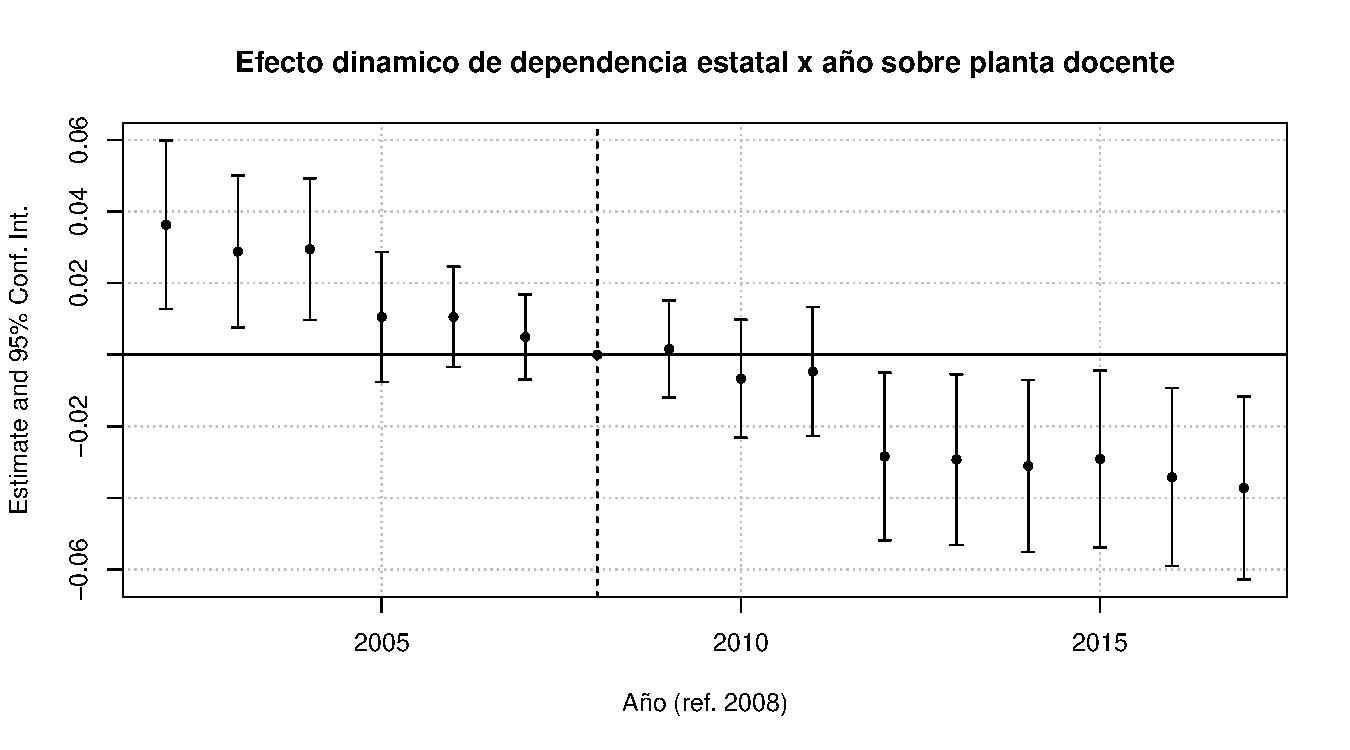
\includegraphics[width=0.7\textwidth,page=1]{figures/mecanismo_planta_docente.pdf}
\caption{Dynamic effect of pre-recession state-funding dependence on total instructional staff headcount, by year relative to 2008. The temporal signature closely replicates the curricular outcome in Fig.~\ref{fig:recession}: no effect through 2011, then a significant, monotonically growing decline from 2012 onward.}
\label{fig:mechanism}
\end{figure}

By contrast, nominal instructional expenditure showed no corresponding decline; if anything, several nominal expenditure categories rose relatively faster in more dependent institutions, plausibly reflecting enrollment growth or a shift of the funding burden onto tuition. Once we normalize expenditure by FTE enrollment, the picture clarifies: operations-and-maintenance spending per student fell significantly in more dependent institutions ($b=-0.025$, $p=0.019$)--consistent with deferred-maintenance being among the first categories cut in fiscal downturns--while instructional expenditure per student showed no significant change ($b=+0.007$, $p=0.449$). Read together with the staffing result, this indicates that institutions largely protected the level of instructional spending per student while reducing the number of instructional staff delivering it--plausibly through hiring freezes, non-replacement of departing faculty, and increased teaching loads--a form of adjustment that would not appear in expenditure data but would directly erode the organizational capacity (faculty time, administrative bandwidth for curriculum committees) needed to revise curricular content.

\subsection*{A second, partly independent test of the resource channel}

The recession design rests on a single natural experiment. To gauge whether the resource mechanism is a general property of the data or an artifact of 2008 specifically, we re-estimate its central prediction using an entirely different source of variation: year-over-year growth in each institution's own real state appropriations (2002--2017), interacted with no single event date, so that a cut in \emph{any} year is allowed to predict slower adoption and abandonment the following year. Across the full panel, a one-standard-deviation larger appropriations cut predicts significantly higher abandonment the following year ($b=-0.0046$ on log-growth, $p=0.027$); the corresponding adoption coefficient is small and not significant ($p=0.63$). When the 2008--2011 window is excluded entirely, the abandonment coefficient falls by roughly a third and loses conventional significance ($b=-0.0033$, $p=0.169$). We read this as partial, not full, independent corroboration: the abandonment channel is detectable in year-to-year variation beyond the recession, but most of its identifying power still comes from the 2008 shock, and the adoption channel does not replicate in this noisier, event-free specification. A future test exploiting a second large, discrete resource shock--rather than continuous year-to-year variation, which is more exposed to reverse causality and measurement error in short-run appropriations data--would be needed to fully separate the general resource mechanism from a 2008-specific one.

\section*{Discussion}

The standard status-cascade account of organizational diffusion predicts that prestigious institutions should be the first to update their offerings toward emerging occupational skill demands, with the rest of the field following at a lag set by relative status. Our associational baseline reproduces this prediction cleanly, and it is the pattern that a large literature on organizational status and diffusion would lead us to expect \parencite{podolny1993, phillipszuckerman2001, clauset2015}. Yet across five distinct designs that isolate plausibly exogenous variation in institutional status--differing in their source of identifying variation, their assumptions, and their vulnerabilities--we find no design in which this status effect survives. Two additional designs (regression discontinuity on institutional research intensity) failed for an interesting reason of their own: not because status has no effect, but because Carnegie's true, multi-dimensional assignment rule does not produce a sufficiently sharp local discontinuity in any proxy we could construct from public data, a limitation we report transparently rather than paper over.

What does survive causal scrutiny is a resource-dependence account. Using real, institution-level state-appropriation data rather than a coarse public/private proxy, we show that fiscal dependence on state government predicts significantly slower curricular adoption and abandonment following the 2008 recession, with a lagged, monotonically strengthening temporal signature that we are able to trace to a parallel decline in instructional staffing rather than in instructional spending. This is, to our knowledge, among the first demonstrations that state disinvestment in public higher education has consequences not just for access, cost, and completion--the outcomes on which this literature has traditionally focused \parencite{demingwalters2017}--but for the substantive content of what is taught.

These results speak directly to the comparison that motivated this study: work on academic status hierarchies, most influentially the demonstration that faculty hiring networks are steep and self-reinforcing \parencite{clauset2015}, has established that prestige structures \emph{who} moves through the academic system. Our results suggest that this same hierarchy does not equally structure \emph{what} is taught: curricular content--at least along the occupationally relevant skill dimension we study--appears to be governed less by an institution's position in the prestige hierarchy than by its fiscal position vis-\`a-vis the state. This is a meaningful qualification of status-cascade accounts of organizational diffusion more broadly \parencite{strangsoule1998, dimaggiopowell1983}: status and resources are often treated as complementary or even interchangeable predictors of organizational dynamism, but where they can be separated--as the natural experiments here allow--only the latter shows a causal signature.

Several limitations bound these conclusions. First, our identification of the resource channel, while triangulated across staffing and normalized expenditure data, remains a single natural experiment (the 2008 recession); replication using other resource shocks--state policy changes, endowment shocks, enrollment-driven revenue swings--would strengthen external validity. Second, our network instrument relies on a structural-equivalence proxy network rather than observed social or administrative ties between institutions; a genuine peer network (for instance, built from the same faculty-hiring data that motivated our institutional comparison to Clauset et al.\ \parencite{clauset2015}) could sharpen this design considerably, and we make a preliminary crosswalk to that data available for future work. Third, the regression-discontinuity failures, while informative about the limits of publicly available Carnegie proxies, mean we cannot rule out a status effect operating specifically at the research-intensity threshold with a magnitude too small for our design to detect; we report this honestly as an inconclusive rather than a null result. Fourth, our analysis is confined to the United States and to the 2000--2017 period; whether the resource-over-status pattern generalizes to other national higher-education systems, with different funding architectures, is an open question.

Occupations, tasks, and now curricula have each been shown to be structured by organizational position rather than by pure functional need. Our results suggest that, at least for the diffusion of occupationally relevant skills into higher-education curricula, the operative dimension of that structure is fiscal, not reputational.

\section*{Methods}

\subsection*{Data sources}

We link four publicly available administrative data sources at the institution (\texttt{UnitID}) level. (i) The Course-Skill Atlas \parencite{javadiansabet2024} provides syllabus-level relevance scores for 2,412 O*NET Detailed Work Activities across $\sim$3 million U.S.\ course syllabi, 2000--2017, each linked to an institution and a field-of-study category (62 categories). (ii) The Carnegie Classification longitudinal file (1973--2021) provides institutional classification codes on a fixed external revision schedule (vintages in 2000, 2005, 2010, 2015 within our window), institutional-system merger records, and continuous covariates (research doctorates granted, degrees conferred, graduate enrollment) used to construct the propensity index in our second regression-discontinuity attempt. (iii) IPEDS graduate-count records provide 2-digit CIP-code enrollment by institution and year, used to construct a field-cip crosswalk and a discipline-level prestige-concentration index. (iv) IPEDS Finance, Human Resources (Employees by Assigned Position), and Fall Enrollment components provide institution-year state-appropriation revenue, functional expenditure by category, instructional staff headcount, and full-time-equivalent enrollment, 2001--2017.

\subsection*{RCA-based adoption and abandonment}

For each institution$\times$field cell $c$, skill $p$, and year $t$, we aggregate syllabus-level relevance scores to $X_{c,p,t}$ and compute $\mathrm{RCA}_{c,p,t}$ as defined in Results. A cell adopts skill $p$ at $t$ if $\mathrm{RCA}_{c,p,t-1} < 1 \leq \mathrm{RCA}_{c,p,t}$; it abandons $p$ at $t$ if $\mathrm{RCA}_{c,p,t-1} \geq 1 > \mathrm{RCA}_{c,p,t}$. Risk sets are defined separately for the two flows--cells not yet specialized in $p$ are at risk of adoption; cells already specialized are at risk of abandonment--allowing re-adoption after abandonment (no absorbing-state restriction). We restrict our event-history and quasi-experimental analyses to the 100 skills with the largest \emph{baseline} (2000--2001 only) asymmetry in specialization rates between R1 and non-R1 institutions (``frontier'' skills). Fixing this selection to the two years preceding the 2001--2017 outcome window, rather than recomputing it over the full panel, ensures the skill set is temporally prior to and independent of the adoption and abandonment events it is used to study; selecting on asymmetry computed across the full panel would let outcome-period dynamics contaminate the selection criterion. The two selection rules agree on 59 of the 100 skills; results are qualitatively unchanged under the corrected, baseline-only selection (Results).

\subsection*{Skill taxonomy}

We classify each analytic skill into one of three types by combining an external functional-domain classification with an internally estimated specificity split. Functional domain (Socio-Cognitive vs.\ Sensory-Physical) is assigned from the official O*NET Content Model: each Detailed Work Activity maps to a parent Generalized Work Activity element ID, and element IDs beginning ``4.A.3'' (Work Output, officially defined as physical activities and equipment/vehicle operation) are coded Sensory-Physical, while ``4.A.1'' (Information Input), ``4.A.2'' (Mental Processes), and ``4.A.4'' (Interacting with Others) are coded Socio-Cognitive; the match rate against our 2,070 baseline-eligible skills is 99.9\%. We initially attempted to classify domain endogenously, following the co-specialization-network-plus-community-detection method used for occupational skill polarization, applied to our institution$\times$field specialization matrix in place of an occupation$\times$skill matrix. This recovered two Louvain communities that did not correspond to a cognitive/physical split (e.g., ``Develop financial analysis methods'' and ``Give medications or immunizations'' were assigned to the same or opposite clusters in a manner inconsistent with task content), because co-specialization in our setting is organized by disciplinary curricular bundling (which skills a given academic program teaches together) rather than by the functional content of the activity itself--a structural difference from occupations, where task profiles are directly organized by job function. We therefore report the endogenous attempt as a documented negative result and use the external O*NET classification throughout. Within the Socio-Cognitive domain, we split skills at the within-domain median of a nestedness-contribution score $c_s$ (the change in a matrix-level NODF nestedness index when a skill is removed from the baseline institution$\times$field specialization matrix, computed via a fully vectorized pairwise-overlap formulation for computational tractability), yielding General (above median) and Specialized (below median) subclasses, in the spirit of prior nestedness-based skill-specificity measures.

\subsection*{Associational baseline}

The baseline model is a discrete-time complementary log-log hazard regression of the adoption (resp.\ abandonment) indicator on standardized system-wide exposure to elite and non-elite adopters of the same skill in the prior year, an institutional prestige measure (binary Carnegie R1 status, or an ordinal 0--3 prestige tier and a continuous discipline-level prestige-concentration index in the alternative specification), and institution$\times$field and year fixed effects, with standard errors clustered by institution.

\subsection*{Quasi-experimental designs}

\emph{Carnegie reclassification.} We define an institution's treatment cohort as the first year in which its ordinal prestige tier increases (or decreases) and does not subsequently revert for the remainder of the panel (``clean'' transitions), excluding institutions that were already at the top tier throughout. We estimate $\mathrm{evento}_{ijt} \sim \mathrm{sunab}(\mathrm{cohort}_i, t) + \mathbf{X}_{ijt} \mid \alpha_i + \alpha_j + \alpha_t$ using the interaction-weighted estimator of \textcite{sunabraham2021}, with never-treated institutions as controls, and separately estimate a generalized synthetic control \parencite{xu2017} on the institution$\times$year adoption and abandonment rate, with cross-validated factor number and parametric bootstrap inference.

\emph{Regression discontinuity.} In the first attempt, the running variable is research doctorates granted (2015 Carnegie vintage, Doctoral institutions only); in the second, it is the linear predictor of a logistic regression of R1 status on research doctorates, total degrees, graduate full- and part-time enrollment, with a natural cutoff at predicted probability 0.5. Both are estimated with local-polynomial bias-corrected inference and data-driven bandwidth selection \parencite{calonico2014}, with a manipulation test on the running variable \parencite{cattaneo2020density}.

\emph{Network instrument.} We construct a directed $k$-nearest-neighbor ($k=10$) network within Carnegie classification groups, using standardized baseline (2000) log-enrollment, prestige tier, and control type as the similarity space. Direct-peer exposure is the lagged mean adoption (resp.\ abandonment) rate among an institution's $k$ nearest neighbors; the instrument is the lagged mean rate among neighbors' neighbors excluding an institution's own direct neighbors, exploiting the network's non-transitivity. We estimate two-stage least squares with institution and year fixed effects and three-way appropriate clustering.

\emph{Mergers.} Treatment cohort is the first year in which an institution appears as the acquiring party (\texttt{MergeInto\_Link}) in the Carnegie longitudinal file; estimation otherwise follows the reclassification event-study.

\emph{State-funding dependence.} We compute institution-year state-appropriations share of total revenue from IPEDS Finance (form F1A for public, GASB-reporting institutions; F2 for private nonprofits, FASB-reporting; F3 for private for-profits), average it over 2005--2007 to construct a standardized pre-recession dependence measure, and estimate $\mathrm{evento}_{ijt} \sim \mathrm{post}2009_t \times \mathrm{dependence}_i + \mathbf{X}_{ijt} \mid \alpha_i + \alpha_j + \alpha_t$, together with a fully dynamic specification interacting calendar year with dependence (reference year 2008).

\emph{Mechanism.} Instructional staffing is total headcount in the ``instructional staff'' occupational category from IPEDS Human Resources (Employees by Assigned Position), harmonized across a 2012 survey redesign that changed the underlying coding scheme (verified to yield exactly one row per institution-year under both coding regimes; see replication code). Functional expenditure by category (instruction, research, academic support, student services, institutional support, operations and maintenance, scholarships, auxiliary enterprises) is drawn from IPEDS Finance form F1A and normalized by IPEDS Fall Enrollment FTE counts (form EFFY) for institutions and years with valid data. Both mechanism outcomes are modeled with the same specification as the state-funding-dependence design.

All models use \texttt{feols}/\texttt{feglm} from the \texttt{fixest} package in R; the generalized synthetic control uses the \texttt{gsynth} package; the regression discontinuities use \texttt{rdrobust} and \texttt{rddensity}.

\subsection*{Use of AI-assisted technologies}
We used Anthropic's Claude (accessed via Claude Code / Cowork) to assist with data pipeline construction, analysis-code development and correctness checking, and to draft and revise manuscript text under close author direction and review. These tools generated no data, results, or scientific claims independently of author specification; all analyses were specified, executed, and interpreted by the authors, who reviewed all AI-assisted output for accuracy and are solely responsible for the final content.

\section*{Data and materials availability}
The analysis draws on publicly available sources: the Course-Skill Atlas (Figshare, \url{https://figshare.com/articles/dataset/A_national_longitudinal_dataset_of_skills_taught_in_U_S_higher_education_curricula/25632429}), the Carnegie Classification longitudinal public data file, IPEDS Finance, Human Resources, and Fall Enrollment complete data files (\url{https://nces.ed.gov/ipeds}), and the Clauset et al.\ faculty hiring network data (\url{https://aaronclauset.github.io/facultyhiring/}). All derived datasets and analysis code are available in the project repository.

\clearpage
\bibliographystyle{unsrtnat}
\bibliography{references}

\end{document}
